\scanpage{98}
% archive sheet number: 100

2) \uline{Cas carré} $n=4$. On voit que l'on a une $\sigma$ du type $E_1$, et $-\sigma$ est du $=$ type. La $\unsure{2^{\mathrm e}|2}$ correspond aux symétries p. r. aux \deleted{\unsure{segments|sommets}} \inserted{diagonales} du carré du départ. La symétrie par rapport à une \unsure{arête|côté} échange $e_0$ et $e_1$, les invariants et anti-invariants sont resp. engendrés par $e_0+e_1$ et $e_0-e_1$, qui n'engendrent \uline{pas} le \deleted{\unsure{ré|rése}}réseau, donc on est dans le cas $E'_{\unsure{a|1|a'}}$. On a

\figure{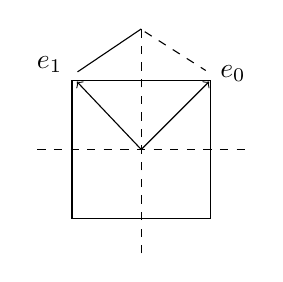
\begin{tikzpicture}[x=.88cm,y=.88cm]
\draw (-1,-1)--(1,-1)--(1,1)--(-1,1)--cycle;
\draw[dashed] (-1.5,0)--(1.6,0) (0,-1.5)--(0,1.75);
\draw[->] (0,0)--(-.93,.98);\draw[->] (0,0)--(.98,.98);
\draw (-.92,1.12)--(0,1.74);\draw[dashed] (.05,1.70)--(.93,1.14);
\node[left] at (-1,1.23) {$e_1$};\node[right] at (1,1.10) {$e_0$};
\end{tikzpicture}}

\margin{\deleted{\unsure{$E$|$E'$}} \unsure{les|cas}}

\[
a'=\frac{Q(e_0-e_1)}{Q(e_0+e_1)}=\deleted{\unsure{4|1|A}}1\quad\text{aussi}
\]

Donc on trouve les types $E_1$ (``sommets'') et $E'_1$ (``côtés'',

3) \uline{Cas hexagonal} $n=6$. \deleted{\unsure{Sy|S}} \uline{Réflexions-sommets}. Les \deleted{\unsure{som|inv}} invariants pour la réflexion p. r. à $\mathbb R u$ sont engendrés par $u$, les anti-invariants par $2v-u$, c'est du type $E'_a$, avec

\figure{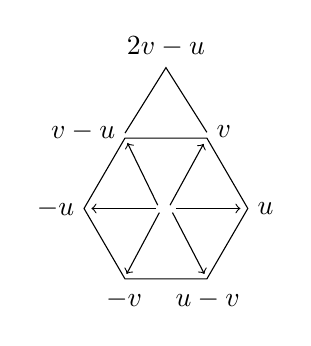
\begin{tikzpicture}[x=1.04cm,y=1.04cm]
\draw (-1,0)--(-.50,.86)--(.50,.86)--(1,0)--(.50,-.86)--(-.50,-.86)--cycle;
\draw (-.50,.92)--(0,1.72)--(.5,.93);
\draw[->] (-.10,.04)--(-.47,.80);\draw[->] (.05,.04)--(.46,.79);\draw[->] (-.12,0)--(-.91,0);\draw[->] (.12,0)--(.91,0);\draw[->] (-.08,-.05)--(-.48,-.80);\draw[->] (.08,-.05)--(.47,-.80);
\node[above] at (0,1.73) {$2v-u$};\node[left] at (-.5,.94) {$v-u$};\node[right] at (.5,.94) {$v$};\node[left] at (-1,0) {$-u$};\node[right] at (1,0) {$u$};\node[below] at (-.51,-.88) {$-v$};\node[below] at (.51,-.88) {$u-v$};
\end{tikzpicture}}

\[
a=\frac{Q(2v-u)}{Q(u)}=\sqrt{3}
\]

\uline{Réflexions-faces} Ce sont les $-\sigma$, on trouve donc $E'_{1/a}=E'_{1/\sqrt{3}}$.

\uline{En résumé}. Dans tous les cas, sauf le cas carré, \deleted{toutes} \inserted{l'une des} \deleted{les} \inserted{les types de} structures réelles sur $X$ sont soit \deleted{du type} $\{E_a,E_{1/a}\}$, \deleted{t cas} soit $\{E'_a,E'_{1/a}\}$ \inserted{avec $a>1$} (le cas hexagonal étant dans le deuxième cas \inserted{avec $a=\sqrt{3}$}), à l'exclusion bien sûr l'une de l'autre. \uline{Dans} le cas carré, l'ens des structures réelles est $\{E_1,E'_1\}$ i.e. il y a à la fois des structures $E$ et $E'$.
